\providecommand{\main}{..}
\documentclass[\main/main.tex]{subfiles}
\begin{document}
\clearpage
\section{CpGobsExp}
\subsection{Metric sample distribution}
The data points seem to follow a \textbf{Beta} distribution.

\begin{figure}
  \includegraphics[width=\textwidth]{distributions/CpGobsExp}
  \caption{Sampling distribution of metric CpGobsExp}
\end{figure}
\subsection{Metric values}
\begin{figure}
  \includegraphics[width=\textwidth]{plot/CpGobsExp}
  \caption{Values of metric CpGobsExp}
\end{figure}

\clearpage
\section{CpGperCpG}
\subsection{Metric sample distribution}
The data points seem to follow a \textbf{Beta} distribution.
\begin{figure}
  \includegraphics[width=\textwidth]{distributions/CpGperCpG}
  \caption{Sampling distribution of metric CpGperCpG}
\end{figure}
\subsection{Metric values}
\begin{figure}
  \includegraphics[width=\textwidth]{plot/CpGperCpG}
  \caption{Values of metric CpGperCpG}
\end{figure}

\clearpage
\section{CpGperGC}
\subsection{Metric sample distribution}
The data points seem to follow a \textbf{Gaussian} distribution.

\begin{figure}
  \includegraphics[width=\textwidth]{distributions/CpGperGC}
  \caption{Sampling distribution of metric CpGperGC}
\end{figure}
\subsection{Metric values}
\begin{figure}
  \includegraphics[width=\textwidth]{plot/CpGperGC}
  \caption{Values of metric CpGperGC}
\end{figure}

\clearpage
\section{DGVCount}
\subsection{Metric sample distribution}
The data points seem to follow a \textbf{Gamma} distribution.

\begin{figure}
  \includegraphics[width=\textwidth]{distributions/DGVCount}
  \caption{Sampling distribution of metric DGVCount}
\end{figure}
\subsection{Metric values}
\begin{figure}
  \includegraphics[width=\textwidth]{plot/DGVCount}
  \caption{Values of metric DGVCount}
\end{figure}

\clearpage
\section{DnaseClusteredHyp}
\subsection{Metric sample distribution}
The data points seem to follow a \textbf{Gamma} distribution.

\begin{figure}
  \includegraphics[width=\textwidth]{distributions/DnaseClusteredHyp}
  \caption{Sampling distribution of metric DnaseClusteredHyp}
\end{figure}
\subsection{Metric values}
\begin{figure}
  \includegraphics[width=\textwidth]{plot/DnaseClusteredHyp}
  \caption{Values of metric DnaseClusteredHyp}
\end{figure}

\clearpage
\section{DnaseClusteredScore}
\subsection{Metric sample distribution}
The data points seem to follow \textbf{slightly} a \textbf{Beta} distribution.

\begin{figure}
  \includegraphics[width=\textwidth]{distributions/DnaseClusteredScore}
  \caption{Sampling distribution of metric DnaseClusteredScore}
\end{figure}
\subsection{Metric values}
\begin{figure}
  \includegraphics[width=\textwidth]{plot/DnaseClusteredScore}
  \caption{Values of metric DnaseClusteredScore}
\end{figure}

\clearpage
\section{EncH3K27Ac}
\subsection{Metric sample distribution}
The data points seem to follow a family of \textbf{Gamma} distributions (a speculation for this distribution could be the different groups from which the data are extracted), we will approximate them to one with a linear combination of the parameters.

\begin{figure}
  \includegraphics[width=\textwidth]{distributions/EncH3K27Ac}
  \caption{Sampling distribution of metric EncH3K27Ac}
\end{figure}
\subsection{Metric values}
\begin{figure}
  \includegraphics[width=\textwidth]{plot/EncH3K27Ac}
  \caption{Values of metric EncH3K27Ac}
\end{figure}

\clearpage
\section{EncH3K4Me1}
\subsection{Metric sample distribution}
The data points seem to follow a family of \textbf{Gamma} distributions (a speculation for this distribution could be the different groups from which the data are extracted), we will approximate them to one with a linear combination of the parameters.

\begin{figure}
  \includegraphics[width=\textwidth]{distributions/EncH3K4Me1}
  \caption{Sampling distribution of metric EncH3K4Me1}
\end{figure}
\subsection{Metric values}
\begin{figure}
  \includegraphics[width=\textwidth]{plot/EncH3K4Me1}
  \caption{Values of metric EncH3K4Me1}
\end{figure}

\clearpage
\section{EncH3K4Me3}
\subsection{Metric sample distribution}
The data points seem to follow a family of \textbf{Gamma} distributions (a speculation for this distribution could be the different groups from which the data are extracted), we will approximate them to one with a linear combination of the parameters.

\begin{figure}
  \includegraphics[width=\textwidth]{distributions/EncH3K4Me3}
  \caption{Sampling distribution of metric EncH3K4Me3}
\end{figure}
\subsection{Metric values}
\begin{figure}
  \includegraphics[width=\textwidth]{plot/EncH3K4Me3}
  \caption{Values of metric EncH3K4Me3}
\end{figure}

\clearpage
\section{GCContent}
\subsection{Metric sample distribution}
The data points seem to be a combination of two \textbf{Gaussian} distributions.

\begin{figure}
  \includegraphics[width=\textwidth]{distributions/GCContent}
  \caption{Sampling distribution of metric GCContent}
\end{figure}
\subsection{Metric values}
\begin{figure}
  \includegraphics[width=\textwidth]{plot/GCContent}
  \caption{Values of metric GCContent}
\end{figure}

\clearpage
\section{GerpRS}
\subsection{Metric sample distribution}
The data points seem to follow a family of \textbf{Gamma} distributions (a speculation for this distribution could be the different groups from which the data are extracted), we will approximate them to one with a linear combination of the parameters.

\begin{figure}
  \includegraphics[width=\textwidth]{distributions/GerpRS}
  \caption{Sampling distribution of metric GerpRS}
\end{figure}
\subsection{Metric values}
\begin{figure}
  \includegraphics[width=\textwidth]{plot/GerpRS}
  \caption{Values of metric GerpRS}
\end{figure}

\clearpage
\section{GerpRSpv}
\subsection{Metric sample distribution}
The data points seem to follow a family of \textbf{Gamma} distributions (a speculation for this distribution could be the different groups from which the data are extracted), we will approximate them to one with a linear combination of the parameters.

\begin{figure}
  \includegraphics[width=\textwidth]{distributions/GerpRSpv}
  \caption{Sampling distribution of metric GerpRSpv}
\end{figure}
\subsection{Metric values}
\begin{figure}
  \includegraphics[width=\textwidth]{plot/GerpRSpv}
  \caption{Values of metric GerpRSpv}
\end{figure}

\clearpage
\section{ISCApath}
\subsection{Metric sample distribution}
The data points seem to follow a \textbf{Gamma} distribution.

\begin{figure}
  \includegraphics[width=\textwidth]{distributions/ISCApath}
  \caption{Sampling distribution of metric ISCApath}
\end{figure}
\subsection{Metric values}
\begin{figure}
  \includegraphics[width=\textwidth]{plot/ISCApath}
  \caption{Values of metric ISCApath}
\end{figure}

\clearpage
\section{commonVar}
\subsection{Metric sample distribution}
The data points seem to follow an \textbf{Exponential Weibull} distribution.
\begin{figure}
  \includegraphics[width=\textwidth]{distributions/commonVar}
  \caption{Sampling distribution of metric commonVar}
\end{figure}
\subsection{Metric values}
\begin{figure}
  \includegraphics[width=\textwidth]{plot/commonVar}
  \caption{Values of metric commonVar}
\end{figure}

\clearpage
\section{dbVARCount}
\subsection{Metric sample distribution}
The data points seem to follow a \textbf{Gamma} distribution.

\begin{figure}
  \includegraphics[width=\textwidth]{distributions/dbVARCount}
  \caption{Sampling distribution of metric dbVARCount}
\end{figure}
\subsection{Metric values}
\begin{figure}
  \includegraphics[width=\textwidth]{plot/dbVARCount}
  \caption{Values of metric dbVARCount}
\end{figure}

\clearpage
\section{fantom5Perm}
\subsection{Metric sample distribution}
The data points seem to follow a \textbf{Gamma} distribution.

\begin{figure}
  \includegraphics[width=\textwidth]{distributions/fantom5Perm}
  \caption{Sampling distribution of metric fantom5Perm}
\end{figure}
\subsection{Metric values}
\begin{figure}
  \includegraphics[width=\textwidth]{plot/fantom5Perm}
  \caption{Values of metric fantom5Perm}
\end{figure}

\clearpage
\section{fantom5Robust}
\subsection{Metric sample distribution}
The data points seem to follow a \textbf{Gamma} distribution.

\begin{figure}
  \includegraphics[width=\textwidth]{distributions/fantom5Robust}
  \caption{Sampling distribution of metric fantom5Robust}
\end{figure}
\subsection{Metric values}
\begin{figure}
  \includegraphics[width=\textwidth]{plot/fantom5Robust}
  \caption{Values of metric fantom5Robust}
\end{figure}

\clearpage
\section{fracRareCommon}
\subsection{Metric sample distribution}
The data points seem to follow an \textbf{Beta} distribution.

\begin{figure}
  \includegraphics[width=\textwidth]{distributions/fracRareCommon}
  \caption{Sampling distribution of metric fracRareCommon}
\end{figure}
\subsection{Metric values}
\begin{figure}
  \includegraphics[width=\textwidth]{plot/fracRareCommon}
  \caption{Values of metric fracRareCommon}
\end{figure}

\clearpage
\section{mamPhastCons46way}
\subsection{Metric sample distribution}
The data points seem to follow a \textbf{Gamma} distribution.

\begin{figure}
  \includegraphics[width=\textwidth]{distributions/mamPhastCons46way}
  \caption{Sampling distribution of metric mamPhastCons46way}
\end{figure}
\subsection{Metric values}
\begin{figure}
  \includegraphics[width=\textwidth]{plot/mamPhastCons46way}
  \caption{Values of metric mamPhastCons46way}
\end{figure}

\clearpage
\section{mamPhyloP46way}
\subsection{Metric sample distribution}
The data points seem to follow a \textbf{Gaussian} distribution.

\begin{figure}
  \includegraphics[width=\textwidth]{distributions/mamPhyloP46way}
  \caption{Sampling distribution of metric mamPhyloP46way}
\end{figure}
\subsection{Metric values}
\begin{figure}
  \includegraphics[width=\textwidth]{plot/mamPhyloP46way}
  \caption{Values of metric mamPhyloP46way}
\end{figure}

\clearpage
\section{numTFBSConserved}
\subsection{Metric sample distribution}
The data points seem to follow a \textbf{exponential} distribution.

\begin{figure}
  \includegraphics[width=\textwidth]{distributions/numTFBSConserved}
  \caption{Sampling distribution of metric numTFBSConserved}
\end{figure}
\subsection{Metric values}
\begin{figure}
  \includegraphics[width=\textwidth]{plot/numTFBSConserved}
  \caption{Values of metric numTFBSConserved}
\end{figure}

\clearpage
\section{priPhastCons46way}
\subsection{Metric sample distribution}
The data points seem to follow a \textbf{Gamma} distribution.

\begin{figure}
  \includegraphics[width=\textwidth]{distributions/priPhastCons46way}
  \caption{Sampling distribution of metric priPhastCons46way}
\end{figure}
\subsection{Metric values}
\begin{figure}
  \includegraphics[width=\textwidth]{plot/priPhastCons46way}
  \caption{Values of metric priPhastCons46way}
\end{figure}

\clearpage
\section{priPhyloP46way}
\subsection{Metric sample distribution}
The data points seem to follow an \textbf{Beta} distribution.
\begin{figure}
  \includegraphics[width=\textwidth]{distributions/priPhyloP46way}
  \caption{Sampling distribution of metric priPhyloP46way}
\end{figure}
\subsection{Metric values}
\begin{figure}
  \includegraphics[width=\textwidth]{plot/priPhyloP46way}
  \caption{Values of metric priPhyloP46way}
\end{figure}

\clearpage
\section{rareVar}
\subsection{Metric sample distribution}
The data points seem to follow an \textbf{Beta} distribution.
\begin{figure}
  \includegraphics[width=\textwidth]{distributions/rareVar}
  \caption{Sampling distribution of metric rareVar}
\end{figure}
\subsection{Metric values}
\begin{figure}
  \includegraphics[width=\textwidth]{plot/rareVar}
  \caption{Values of metric rareVar}
\end{figure}

\clearpage
\section{verPhastCons46way}
\subsection{Metric sample distribution}
The data points seem to follow a \textbf{Gamma} distribution.

\begin{figure}
  \includegraphics[width=\textwidth]{distributions/verPhastCons46way}
  \caption{Sampling distribution of metric verPhastCons46way}
\end{figure}
\subsection{Metric values}
\begin{figure}
  \includegraphics[width=\textwidth]{plot/verPhastCons46way}
  \caption{Values of metric verPhastCons46way}
\end{figure}

\clearpage
\section{verPhyloP46way}
\subsection{Metric sample distribution}
The data points seem to follow a \textbf{Gaussian} distribution.
\begin{figure}
  \includegraphics[width=\textwidth]{distributions/verPhyloP46way}
  \caption{Sampling distribution of metric verPhyloP46way}
\end{figure}
\subsection{Metric values}
\begin{figure}
  \includegraphics[width=\textwidth]{plot/verPhyloP46way}
  \caption{Values of metric verPhyloP46way}
\end{figure}

\end{document}
